\documentclass[lettersize,journal,12pt]{IEEEtran}
\usepackage{fontspec}
\usepackage{amsmath,amsfonts}
\usepackage{algorithmic}
\usepackage{algorithm}
\usepackage{array}
\usepackage[caption=false,font=normalsize,labelfont=sf,textfont=sf]{subfig}
\usepackage{textcomp}
\usepackage{stfloats}
\usepackage{url}
\usepackage{verbatim}
\usepackage{xeCJK}
\usepackage{lettrine}
\usepackage{graphicx}
\usepackage{titling}
\usepackage{titlesec}
\usepackage{balance}
\usepackage{textcase}
\usepackage{setspace}
\setmainfont{Times New Roman}[SmallCapsFont=TeX Gyre Termes:+smcp]
% rule to break words
\hyphenation{}
\def\BibTeX{{\rm B\kern-.05em{\sc i\kern-.025em b}\kern-.08em
T\kern-.1667em\lower.7ex\hbox{E}\kern-.125emX}}
\pretitle{\begin{center}\fontsize{16}{18}\selectfont\bfseries}
\posttitle{\end{center}}
\preauthor{\begin{center}\fontsize{10}{12}\selectfont}
\postauthor{\end{center}}
\predate{\begin{center}\fontsize{10}{12}\selectfont}
\postdate{\end{center}}
\titleformat{\section}
{\filcenter\fontsize{14}{16}\bfseries\uppercase}
{\thesection}
{1em}
{}
\renewenvironment{abstract}
{\fontsize{12}{14}\textit{\textbf{\abstractname---}}\bfseries\ignorespaces}
{}
\renewenvironment{IEEEkeywords}
{\fontsize{12}{14}\textit{\textbf{Keywords---}}\bfseries\ignorespaces}{}
\begin{document}
\onehalfspacing
\title{Unveiling the PageRank Algorithm: Principles, Performance, and Enhancements}
\author{Wu Zelin, Wu Zekai, Li Pengda
	\thanks{We should thank Ms.Ye here}}

\maketitle\thispagestyle{headings}
\markboth{10225101428 吴泽霖\quad10225101429 武泽恺\quad10225101460 李鹏达}{}%

\begin{abstract}
	This is the abstract area. We should write a very nb abstract here.
\end{abstract}

\begin{IEEEkeywords}
	Keyword1, Keyword2, Keyword3
\end{IEEEkeywords}


\section{Introduction}
\lettrine{I}{n}
the past decade,the field of information technology has darmatically changed.One of the force is the super robust and fast
Web search algorithms which are capable of handling massive and enomorous data.
Amony many of these algorithms,PageRank is the fundamental and the most commonly used algorithm in the web and information retrieval.
\\
\indent PageRank is algorithm developed by Larry Page and Sergey Brin in the late 1990s to measure the importance of web pages. 
It was originally created for the Google search engine and is named after one of the founder of Google Larry Page.
Google search engine uses the algorithm to analyze the relevance and importance of web pages and regard it as one of the factors
 to evaluate the effectiveness of web page optimization.Although Other algorithms are applied to rank web pages nowadays,the PageRank 
 is also one of the oldest and famous algorithms.
\\
\indent In this paper, we make the following simple insights and research:
\begin{itemize}
	\item The operation mode of the PageRank and the principles it used
	\item PageRank's algorithmic determinism of the importance of the web pages
	\item The impact of damping factors on search results and page rankings
	\item Explore the possibility of other factors that can improve PageRank performance except for link analysis
\end{itemize}
\indent In the next section,PageRank is briefly reviewed and analyzed.
\lettrine{W}{ith}
the proliferation of the Internet, the explosively increasing amount of web pages on the World Wide Web has created the demand for the web searching engines with high-efficiency and high-effectiveness. 
For the biggest search engine company Google, which held a global market share of 93.18\% until March 2023, it is of primary significance to develop a powerful search algorithm to provide users with the most relevant and useful results in the shortest time. 
Previous studies on web search algorithms have proven that TF-IDF algorithm and BM25 algorithm were efficient and effective in the early days of the Internet. 
However, these algorithms have been unable to meet the growing demand of users. 
The users' search queries are becoming diversified and the web pages are becoming complex.
According to the statistics, the number of web pages has increased to 130 trillion in 2016, which means that the amount of web pages has increased by 130 times in 20 years and it takes longer time to search for the most relevant web pages.
To overcome the aformentioned chanllenge, Google has developed a state-of-the-art algorithm called PageRank, which is currently a fundamental algorithm in web search and redefine how we navigate web search.
PageRank is a significant algorithm in web search and information retrieval. It is an algorithm developed by Larry Page and Sergey Brin in the late 1990s to measure the importance of web pages. 
It was originally created for the Google search engine. 
This essay aims to investigate the PageRank algorithm's implementation principles and effectiveness, exploring potential enhancements. 

\section{Related Work}

We should introduce some nb works here.
And we should cite some papers here.

\subsection{Subsection 1}

In this section we should introduce some nb works here.

\subsection{Subsection 2}

This is a simple subsection too.

\section{Main Method and Theory}

We should introduce our methods and Theories here.

\subsection{Subsection 1}

This is a simple subsection. 
We can make a citation here. \cite{ref1}

\figurename~\ref{fig1} is a figure. You can see it at the top of the page.

\begin{figure}[!t]
	\centering
	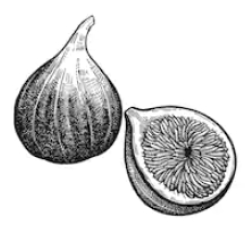
\includegraphics[width=2.5in]{images/fig1.png}
	\caption{This is a figure.}
	\label{fig1}
\end{figure}

\subsection{The 3rd Section 2nd Subsection}

This is a simple subsection too.
\section{Experiment}

This is a simple section.
\subsection{The 4th Section 1st Subsection}

This is a simple subsection.

This is an equation:

\begin{equation}
	\label{eq:1}
	e^{\pi i} + 1 = 0
\end{equation}
You can ref it by see\eqref{eq:1}.

\subsection{The 4th Section 2nd Subsection}

This is a simple subsection too.

This is a algorithm:

\begin{algorithm}[H]
	\caption{Weighted Tanimoto ELM.}\label{alg:alg1}
	\begin{algorithmic}
		\STATE
		\STATE {\textsc{TRAIN}}$(\mathbf{X} \mathbf{T})$
		\STATE \hspace{0.5cm}$ \textbf{select randomly } W \subset \mathbf{X}  $
		\STATE \hspace{0.5cm}$ N_\mathbf{t} \gets | \{ i : \mathbf{t}_i = \mathbf{t} \} | $ \textbf{ for } $ \mathbf{t}= -1,+1 $
		\STATE \hspace{0.5cm}$ B_i \gets \sqrt{ \textsc{max}(N_{-1},N_{+1}) / N_{\mathbf{t}_i} } $ \textbf{ for } $ i = 1,...,N $
		\STATE \hspace{0.5cm}$ \hat{\mathbf{H}} \gets  B \cdot (\mathbf{X}^T\textbf{W})/( \mathbb{1}\mathbf{X} + \mathbb{1}\textbf{W} - \mathbf{X}^T\textbf{W} ) $
		\STATE \hspace{0.5cm}$ \beta \gets \left ( I/C + \hat{\mathbf{H}}^T\hat{\mathbf{H}} \right )^{-1}(\hat{\mathbf{H}}^T B\cdot \mathbf{T})  $
		\STATE \hspace{0.5cm}\textbf{return}  $\textbf{W},  \beta $
		\STATE
		\STATE {\textsc{PREDICT}}$(\mathbf{X} )$
		\STATE \hspace{0.5cm}$ \mathbf{H} \gets  (\mathbf{X}^T\textbf{W} )/( \mathbb{1}\mathbf{X}  + \mathbb{1}\textbf{W}- \mathbf{X}^T\textbf{W}  ) $
		\STATE \hspace{0.5cm}\textbf{return}  $\textsc{sign}( \mathbf{H} \beta )$
	\end{algorithmic}
	\label{alg1}
\end{algorithm}

\section{Results}

This is the results area. We should write some very nb results here.

\section{Conclusion}

This is the conclusion area. We should write a very nb conclusion here.



\begin{thebibliography}{1}

	\bibitem{ref1}
	S. Zhan, S. Li and W. Wang, {\it{A Very Nb Book}}. Shanghai, P.R.C., East China Normal  Univ. Press, 2022.

\end{thebibliography}

\end{document}


